\chapter{Problemas}
\label{ch:problemas}

Los problemas a resolver pueden ser de diferente temática o
categoría. Y tu solución entregada puede obtener diferentes
resultados. El objetivo es conseguir siempre el Accepted (\texttt{AC}), pero
dependiendo del concurso puedes obtener diferentes resultados en caso
de fallar en la respuesta entregada, algunos serían:

\begin{itemize}
\item Run Time Error (\texttt{RE} o \texttt{RTE}). La solución ha
  sufrido algún problema durante su ejecución y se ha anulado.
\item Wrong Answer (\texttt{WA}). La solución ha generado una
  respuesta incorrecta.
\item Time Limit (\texttt{TL}). La solución se ha mantenido durante
  demasiado tiempo en ejecución y ha sido abortada.
\item Compilation Error (\texttt{CE}). La solución enviada no ha
  compilado.
\end{itemize}

Los problemas a resolver durante los concursos suelen ser aplicaciones
de consola, por lo que reciben los datos de ejecución a través de la
entrada estándar, y envían los resultados a la salida estándar.\\

Los problemas se centran principalmente en cuestiones de algoritmia y
estructuras de datos. Para poder poner a prueba la corrección de las
soluciones de los participantes, la implementación en cuestión debe
probarse con muchos casos de entrada; debido a eso, la entrada de los
programas es multicaso. Esto significa que si, por ejemplo, el
problema consiste en indicar el último dígito del factorial de un
número dado, la entrada de ese problema estará compuesta de muchos
números (``casos'') para que el código de extracción del último dígito
se ponga a prueba muchas veces.\\

Es importante, por lo tanto, que los participantes tengan destreza con
la entrada y salida estándar del lenguaje de programación que
utilicen.\\

Las soluciones de los participantes a los problemas no sólo deben ser
correctas, sino que deben ejecutarse dentro de unos límites de tiempo
razonables. Se deben evitar, en la medida de lo posible,
implementaciones lentas cuando hay otras similares en dificultad de
programación más eficientes en ejecución. También se hace necesario
prestar atención a la complejidad del algoritmo. Algunos problemas se
suelen plantear persiguiendo que se implemente una solución concreta,
y las restricciones de tiempo configuradas en el juez automático
persiguen precisamente impedir que soluciones ineficientes entren en
tiempo.\\

Los siguientes subcapítulos, excepto el primero, corresponden con una
clasificación de los problemas en función del tipo de solución que
requieren. En cada apartado se describe la categoría, se explica los
tipos de algoritmos que se pueden utilizar y se muestra uno o dos
ejemplos del juez online de la Universidad de Valladolid (UVA) y una
posible solución en C/C++. El primer subcapítulo es un breve resumen
de estructuras de datos que podemos encontrar en librerías o debemos
saber cómo implementar y utilizar en el lenguaje de programación que
elijamos.

\section{Estructuras de Datos y Librerías}
\label{sec:datos}

Las estructuras de datos son el mecanismo para almacenar y organizar
los datos con el fin de permitir realizar de manera eficiente
inserciones, búsquedas, eliminaciones, preguntas y
actualizaciones. Ninguna estructura de datos soluciona por sí misma
ningún problema sino el algoritmo que las utiliza. Se deben conocer
las diferentes estructuras de datos para utilizar la más acorde a las
necesidades del problema de modo que se optimicen las operaciones que
más se vayan a realizar.

Por un lado, encontramos estructuras que acostumbran a estar definidas
en librerías. Algunas de estas son:
\begin{itemize}
\item \emph{Array estático}: es la más sencilla de las estructuras y
  se utiliza cuando queremos almacenar una colección secuencial de
  datos de tamaño máximo pequeño y conocido.
\item \emph{Array dinámico}: comúnmente llamado \lst{vector}, realiza
  la misma funcionalidad que el Array estático pero nos ofrece el
  incremento de tamaño de manera automática sin preocuparnos de tener
  que reservar o liberar memoria. Sus operaciones más típicas son
  \lst{push\_back} (añadir al final) , \lst{at} (consultar una posición) y
  permite ser recorrido con iteradores.
\item \emph{Lista enlazada}: normalmente se evita utilizar esta
  estructura en los concursos porque conlleva un tratamiento de
  punteros para acceder a los datos donde es demasiado fácil
  equivocarse. En su lugar se utiliza un \lst{vector} que otorga el
  mismo servicio e incluso es más flexible.
\item \emph{Pila}: se suele utilizar para resolver problemas como el
  cálculo de resultados en notación postfija o comprobar el balanceado
  de paréntesis, Se caracteriza por su funcionamiento \lst{LIFO}
  (último en entrar es el primero en salir). Sus operaciones comunes
  son \lst{push} (añadir), \lst{pop} (obtener el último elemento) y
  \lst{empty} (comprueba si quedan elementos).
\item \emph{Cola}: se utiliza en algoritmos de búsqueda en anchura
  (BFS) y al contrario que la pila su funcionamiento es \lst{FIFO}
  (primero en entrar es el primero en salir). Las operaciones de las
  que se disponen son \lst{push} (añadir al final), \lst{pop} (obtener
  el primer elemento) y \lst{empty} (comprueba si quedan elementos).
\item \emph{Máscara de Bits}: sustituye a los arrays de booleanos ya
  que se puede operar sobre ellos con menor coste en la ejecución
  aunque su uso es más complicado o por lo menos menos intuitivo.
\item \emph{Árbol binario balanceado}: conocidos como \lst{map} o
  \lst{set} en C++ y \lst{TreeMap} o \lst{TreeSet} en Java. Esta
  estructura es capaz de organizar los datos como un árbol de modo que
  en cada subárbol del mismo cuya raíz podemos llamar x cumple que los
  elementos del subárbol de la izquierda de x son menores que x, y los
  elementos del subárbol de la derecha de x son iguales o mayores que
  x.
\item \emph{Montículo (Heap)}: también llamados colas de prioridad, es
  otra forma de organizar en forma de árbol los datos y ofrecerlos
  como si se tratase de una lista de elementos ordenador por su
  prioridad o peso.
\end{itemize}

Por otro lado, los participantes deben ser capaces de implementar
estructuras de datos que no suelen estar en las librerías como son:
\begin{itemize}
\item \emph{Grafos}: una colección de nodos unidos por aristas. Los
  nodos suelen tener la información y las aristas indican
  relaciones. Se pueden implementar de diferentes maneras:
  \begin{itemize}
  \item \emph{Matriz de adyacencia}: Utilizando un array 2D la
    posición [i,j] indica si existe una arista entre el nodo i-ésimo y
    j-ésimo y el peso de la misma.
  \item \emph{Lista de adyacencia}: Habitualmente implementado como un
    vector de vectores de parejas de enteros (vector\lt~vector\lt~pair\lt~
    int, int\gt~\gt~\gt).
  \item \emph{Lista de aristas}: En ocasiones no es necesario
    almacenar los nodos sino sus relaciones por lo que se utiliza una
    lista de parejas de enteros.
  \end{itemize}
\item \emph{Union-Find disjoint set}: es una estructura para modelar
  colecciones de conjuntos disjuntos entre sí que nos permite realizar
  de manera eficiente la búsqueda del set que contiene uno o más
  elementos concretos, la unión de dos conjuntos disjuntos.
\item \emph{Árbol de segmentos}: esta estructura nos permite realizar
  consultas de segmentos dinámicos, por ejemplo saber cuántos
  elementos hay del 5 al 10 y luego del 7 al 25. Cada nodo del árbol
  resultante contiene la información de la suma de sus hijos y si
  quieres un subconjunto de ellos se desciende en el árbol y un
  superconjunto se asciende. De modo que al final te quedas con los
  nodos que completan tu segmento. La dificultad de esta estructura
  reside en la construcción de la misma que puede hacerse de manera
  inteligente mediante programación dinámica.
\end{itemize}

\section{Divide y Vencerás}
\label{sec:divideyvenceras}

Divide y vencerás es un paradigma de resolución de problemas que
pretende descomponer el problema en subproblemas más sencillos de
tratar. Los pasos a seguir son:
\begin{enumerate}
\item Dividir el problema en subproblemas, habitualmente por la mitad.
\item Buscar la solución a estos subproblemas que pueden pasar por
  volver a dividirlos y ahora son mucho más sencillos.
\item Obtener la solución de cada subproblema y generar la solución
  completa final.
\end{enumerate}
Por ejemplo se puede utilizar para realizar búsquedas binarias.

Un problema de esta categoría es:

\lst{10077: The Stern-Brocot Number}\footnote{\url{https://uva.onlinejudge.org/external/100/10077.pdf}}.
En resumen el problema dice que podemos construir un árbol binario de
fracciones $\frac{n}{m}$ tal que m y n son positivos y primos entre sí, como
el de la Figura~\ref{fig:problema10077}.

\begin{figure}[h]
\hrule\smallskip
\begin{center}
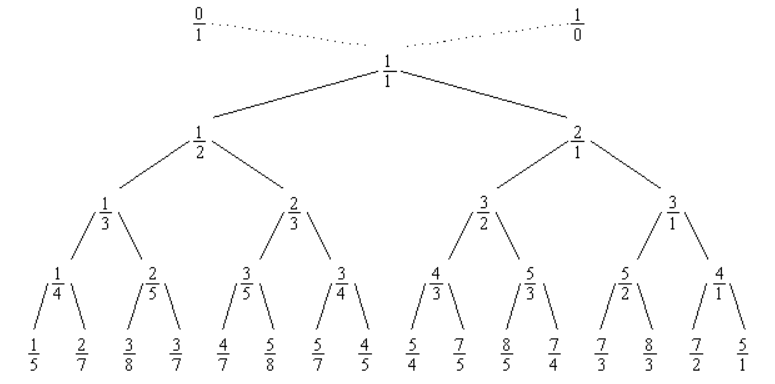
\includegraphics[width=1\textwidth]{fig/problema10077.png}
\end{center}
\caption{Árbol binario del problema 10077}
\label{fig:problema10077}
\hrule
\end{figure}

Y nos pide que indiquemos cual es el recorrido que hay que hacer desde
la raíz para encontrar una fracción concreta, donde \lst{L} significa
descender por la izquierda y \lst{R} por la derecha. Tenemos que
realizar una búsqueda en un árbol binario NO balanceado (u
ordenado). Por tanto se puede simplificar con la búsqueda del elemento
en cada subárbol. La solución en C++ podría ser:

\medskip
\begin{lstlisting}
int Compare(int a, int b, int c, int d) {
  if (a==c && b==d) 
    return 0;
  return (a*d > b*c)? 1: -1;
}
int main() {
  int n, m;
  while (scanf("%d %d", &n, &m)!=EOF){
    if (n==1 && m==1) 
      break;
    int a = 0, b = 1, c = 1, d = 0;
    while (1) {
      int x = a + c, y = b + d;
      int cmp = Compare(n, m, x, y);
      if (cmp==0) break;
      if (cmp==1) {
        printf("R");
        a = x;
        b = y;
      } else {
        printf("L");
        c = x;
        d = y;
      }
    }
    printf("\n");
  }
}
\end{lstlisting}

En la solución no llegamos a guardar el árbol binario sino que
simplemente realizamos una búsqueda binaria normal. Comparando el
elemento buscado ($\frac{n}{m}$) con el del nodo actual recién
calculado ($\frac{x}{y}$), si somos el mismo habremos terminado y si somos
mayores (n*m > x*y) bajaremos por el lado de la derecha y lo
escribiremos. Si somos menores haremos lo mismo pero por la izquierda.

\section{Programación Dinámica}
\label{sec:dp}

La programación dinámica (\lst{DP}) es un paradigma de programación
que se utiliza cuando el problema a resolver tiene subproblemas
superpuestos, es decir, para resolver un problema necesitas resolver
varias veces un mismo subproblema. La DP trata de evitar recalcular
subproblemas. 

Un problema de esta categoría podría ser:

\lst{10465: Homer Simpson}\footnote{\url{http://uva.onlinejudge.org/external/104/10465.html}}.

El problema dice que Homer Simpson quiere comer el máximo número
posible de dos tipos de hamburguesas sabiendo que un tipo tarda m
segundos y otro tarda n teniendo un total de \emph{t} segundos para
comer. Una de las cosas más interesantes y quizá más divertidas de los
problemas es que la tarea a realizar suele estar escondida en
literatura, a veces divertida, como este caso, y en otras ocasiones
formativa. Hay que saber leer en diagonal pero con cuidado ya que
muchas veces la clave del ejercicio está escondida en esa literatura.

\begin{lstlisting}
int main () {
  int m, n, t;
  while ( scanf ("%d %d %d", &m, &n, &t) != EOF ) 
  {
    int times [10000 + 10];
    memset (times, 0, sizeof (times));
    if ( m > n ) 
      swap (m, n);
    times [m] = 1;
    times [n] = 1;
    for ( int i = m; i <= t; i++ ) {
      if ( times [i] ) {
        if ( i + m <= t ) 
          times [i + m] = max ( times [i + m], times [i] + 1);
        if ( i + n <= t ) 
          times [i + n] = max ( times [i + n], times [i] + 1);
      }
    }
\end{lstlisting}

En este fragmento de código podemos observar cómo se rellena la tabla
de programación dinámica llamada en esta ocasión \emph{times} comenzando
por m y n, y el resto de casos se rellenan solo si no se ha
solucionado antes con la comprobación \emph{if (times[i])}. La tabla
después de esto tendrá en \emph{times[i]} la cantidad de hamburguesas que
puede tomar en \emph{i} segundos.


\begin{lstlisting}
    if ( times [t] > 0 )
      printf ("%d\n", times [t]);
    else {
      bool printed = false;
      for ( int i = t - 1; i >= 0; i-- ) {
        if ( times [i] > 0 ) {
          printf ("%d %d\n", times [i], t - i);
          printed = true;
          break;
        }
      }
      if ( !printed )
        printf ("0 %d\n", t);
    }
  }
  return 0;
}
\end{lstlisting}

En este segundo fragmento es donde se consulta de los \emph{t} segundos. En
caso de que la cuenta de hamburguesas no ajuste el tiempo exacto
disponible se consulta hasta obtener un tiempo exacto (t = t - 1) y se
escribe, tal y como indica el enunciado, el número de cervezas que
puede tomar Homer en su tiempo sobrante teniendo en cuenta que toma
una cerveza por segundo.


\section{Grafos}
\label{ref:grafos}

Muchos de los problemas de la vida real se pueden clasificar como problemas de grafos. Algunos tienen soluciones eficientes y otros tienen la categoría de “NP” que indica que no se conoce una solución que tarde menos que tiempo exponencial en función a la entrada. El mundo de los grafos es tan amplio que daría lugar a hacer una clasificación dentro de ellos siguiendo por ejemplo estas subcategorías:
\begin{itemize}
\item Búsqueda primero en profundidad (DFS).
\item Búsqueda primero en anchura (BFS).
\item Búsqueda de componentes conexas.
\item Componentes fuertemente conexas.
\item Coloreado de grafos.
\item Ordenación topológica.
\item Grafos bipartitos.
\item Máximo flujo o punto de corte mínimo
\end{itemize}
El problema de ejemplo pertenece a la penúltima categoría: Grafos
bipartitos, BFS y DFS. 

\lst{10004: Bicoloring}\footnote{\url{https://uva.onlinejudge.org/external/100/10004.pdf}}

\begin{lstlisting}
int col[400];
int vis[400];
 
vi g[400];
 
bool dfs(int u){
  vis[u]=1;
  int n=sz(g[u]);
  for0(i,n){
    if(!vis[g[u][i]]){
      col[g[u][i]] = col[u]^1;
      vis[g[u][i]]=1;
      dfs(g[u][i]);
    } else if(col[u] ^ col[g[u][i]]==0)
      return 0;
  }
  return 1;
}

int main() {
  int n,e;
  while(si(n) && n) {
    si(e);
    for0(i,e) {
      int x,y;
      sii(x,y);
      g[x].pb(y);
      g[y].pb(x);
    }
    if(dfs(0)){
      puts("BICOLORABLE.");
    } else {
      puts("NOT BICOLORABLE.");
    }
    for0(i,200) {
      g[i].clear();
    }
    cover(col,0);
    cover(vis,0);
  }
  return 0;
}
\end{lstlisting}


En este código podemos apreciar la función \lst{dfs} que es el
algoritmo puro de búsqueda en profundidad, añadiendo la asignación de
color. Mientras en el main se construye el grafo y se llama a la
búsqueda en profundidad desde el nodo 0, si consigue llegar a todos
con dos colores será bipartito y sino no.\\

Además en el código vemos la utilización de algunas ``funciones'' no
conocidas como son \lst{for0}, \lst{sz}, \lst{cover}, etc. Se tratan
de atajos creados para tardar menos a la hora de programar, suelen
hacerse, en C++, con \emph{\#define}, por ejemplo \lst{for0(i,n)}
corresponde a un \emph{for} con \emph{i} valor inicial \emph{0} hasta
que tenga valor \emph{n}.\\

Otro ejemplo de la última categoría Máximo flujo (Max Flow) podría
ser:

\lst{10594: Data Flow}\footnote{\url{https://uva.onlinejudge.org/external/105/p10594.pdf}}.

Este ejercicio nos plantea una situación de comunicacion entre un
servidor local y el principal, el problema es que todabia no tienen
todo listo pero necesitan mandarla información por diferentes caminos,
aprovechando al máximo la capacidad de la red, para obtener el mínimo
tiempo posible. En este mismo resumen hecho se puede apreciar que
conozco el tipo de problema dado que he hablado de maximizar el flujo
(\lst{MaxFlow}) de datos para minimizar el tiempo (\lst{MinCost}).

\begin{lstlisting}
int main(){
  int N,M,u[5000],v[5000];
  long long cst[5000],D,K;

  while(scanf("%d %d",&N,&M)==2){
    V = 2*N+1;
    for(int i = 0;i<M;++i){
      scanf("%d %d %lld",&u[i],&v[i],&cst[i]);
      --u[i]; --v[i];
    }
    scanf("%lld %lld",&D,&K);
    init();
    add_edge(0,1,D,0);
    
    for(int i = 0;i<N;++i) add_edge(1+2*i,1+2*i+1,INF,0);
    
    for(int i = 0;i<M;++i){
      add_edge(1+2*u[i]+1,1+2*v[i],K,cst[i]);
      add_edge(1+2*v[i]+1,1+2*u[i],K,cst[i]);
    }
        
    mcmf(0,2*N-1);
        
    if(flowVal!=D) printf("Impossible.\n");
    else printf("%lld\n",flowCost);
  }
  
  return 0;
}
\end{lstlisting}


Aprovecho este ejemplo para indicar más información de cómo se
programa para concursos. El algoritmo de \emph{MinCostMaxFlow} es un
algoritmo conocido y que, aunque se trata de un algoritmo interesante
de entender, no es necesario entenderlo para usarlo, solo se necesita
saber qué hace. Por eso, asumimos que tenemos implementado el
algoritmo en la función \lst{mcmf}. El problema nos pide descubrir cuál es
la cantidad máxima de datos que podemos pasar de un punto a otro por
lo que podemos aplicar el algoritmo una vez hemos preparado la
estructura de datos. Por lo que construimos el grafo y listo, problema
resuelto.

\section{Matemáticas}
\label{sec:matematicas}

La existencia de una categoría llamada matemáticas resulta curiosa,
dado que todas las categorías están basadas en modelos matemáticos. En
esta categoría metemos todos aquellos problemas donde aplicar fórmulas
o propiedades conocidas y todos aquellos que consistan en modelar la
realidad. La mayoría de problemas en esta sección se resuelven
\emph{ad-hoc} unos muy sencillos que ocupan unas simples líneas y
otros de mayor complejidad aplicando propiedades de conjuntos por
ejemplo, sería la utilización de números primos y propiedades de
ellos.

El ejemplo de esta sección es uno de los recomendados hacer primero
dado que es el que más usuarios han conseguido solucionar.

\lst{100: The 3n+1 problem}\footnote{\url{https://uva.onlinejudge.org/external/1/100.pdf}}.

En el mismo problema nos dan un pseudo-código (ver
Figura~\ref{fig:problema100}) que podría valer como solución, si no
fuera porque no entra en tiempo, necesita un poco más de enjundia para
tenerlo.

\begin{figure}[h]
\hrule\smallskip
\begin{center}
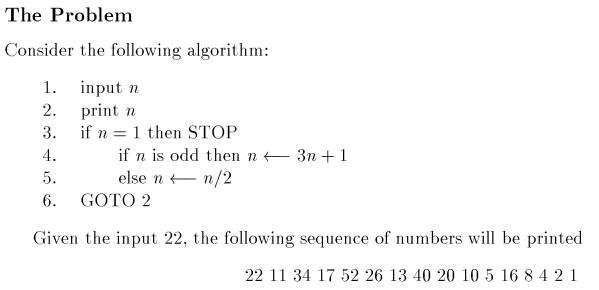
\includegraphics[width=1\textwidth]{fig/problema100.png}
\end{center}
\caption{Pseudo-código del problema 100}
\label{fig:problema100}
\hrule
\end{figure}

\begin{lstlisting}
int main (){
  int i, j;
  while ( scanf ("%d %d", &i, &j) != EOF ) {
    int temp_i = i, temp_j = j;
    if ( i > j ) swap (i, j);
    int max_cycle_length = 0;
    int cycle_length;
    while ( i <= j ) {
      unsigned int n = i;
      cycle_length = 1;
      while ( n != 1 ) {
        if ( n % 2 == 1 ) n = 3 * n + 1;
        else n /= 2;
        cycle_length++;
      }
      if ( cycle_length > max_cycle_length )
        max_cycle_length = cycle_length;
      i++;
    }
    printf ("%d %d %d\n", temp_i, temp_j, max_cycle_length);
  }
  return 0;
}
\end{lstlisting}

La solución surge de aplicar casi directamente el código del enunciado
teniendo cuidado con ciertos casos como que \emph{j} sea menor que \emph{i}.


\section{Procesado de Cadenas de texto}
\label{sec:texto}

Otros problemas se basan en el tratamiento de cadenas de texto
(\emph{string}), puede ser simplemente un tratamiento tedioso pero
sencillo o requerir de estructuras de datos elaboradas para poder
computar sobre ellas. De la primera clase podemos encontrar problemas
que nos digan: ``la entrada consiste en una serie de caracteres
[a-zA-Z], [0-9] y ‘.’ de modo que tienes que comprobar que nunca
suceda que dos números consecutivos sean decrecientes y que en la
cadena no aparezca la palabra ‘hola’'' Esto se puede implementar con
cuidado pero de manera muy sencilla, sin embargo existen otros como la
búsqueda de palíndromos o subcadenas y aplicar algoritmos como
\emph{Knuth-Morris-Pratt} (\lst{KMP}).

\lst{11151: Longest Palindrome}\footnote{\url{https://uva.onlinejudge.org/external/111/p11151.pdf}}.

Consiste en encontrar el palíndromo más largo tal y como indica el
título. Se realiza por medio de programación dinámica y es un
algoritmo conocido y solo hay que llamarlo desde el main parseando
bien la entrada. El algorítmo versa así:

\begin{lstlisting}
int Longest_Palindrome(int lft, int rgt) {
  if(lft==rgt) 
    return 1;
  if(lft>rgt) 
    return 0;

  if(dp[lft][rgt]!=-1) 
    return dp[lft][rgt];

  int ret=0;
  if(s[lft]==s[rgt])
    ret = Longest_Palindrome(lft+1,rgt-1) + 2;
  else
    ret=max(Longest_Palindrome(lft+1,rgt),Longest_Palindrome(lft,rgt-1));
 
  dp[lft][rgt]=ret;
  return dp[lft][rgt];
}
\end{lstlisting}


\section{Geometría Computacional}
\label{sec:geometria}

La geometría computacional aparece múltiples veces en los concursos de
programación y requiere disponer de estructuras donde almacenar
diferentes figuras geométricas y ser capaces de intersecar, unir,
separar, etc. Aunque muchas veces el uso de figuras geométricas puede
simplificarse en aplicar una serie de fórmulas y no hace falta modelar
dichas figuras, solo sus representantes.

Un problema sería 

\lst{460: Overlapping Rectangles}\footnote{\url{https://uva.onlinejudge.org/external/4/460.pdf}}.

Consiste en intersecar dos rectángulos y ver si se superponen.

\begin{lstlisting}
int main() {
  int nTestCases;
  int x1, x2, x3, x4, y1, y2, y3, y4;
  int max1, max2, min1, min2;
  scanf("%d", &nTestCases);
  while(nTestCases--) {
    scanf("%d %d %d %d %d %d %d %d", 
          &x1, &y1, &x2, &y2, &x3, &y3, &x4, &y4);
    max1 = max(x1,x3);
    min1 = min(x2,x4);
    max2 = max(y1,y3);
    min2 = min(y2,y4);    
    if (max1 >= min1 or max2 >= min2) 
      printf("No Overlap\n");
    else 
      printf("%d %d %d %d\n", max1, max2, min1, min2);
    
    if(nTestCases) printf("\n");
  }
  return 0;
}
\end{lstlisting}

En este problema debemos prestar atención para no cometer un error de
presentación (\lst{PE}), lo evitamos con la última linea
\emph{if(nTestCases) printf("\textbackslash{}n");}, ya que debemos poner un intro
después de cada caso menos del último, entonces cuando
\emph{nTestCases} sea \emph{0} no podrá el salto de línea final.
